\begin{frame}
\frametitle{About This Work...}

\emph{Learning-Based Cleansing for Indoor RFID Data}~\cite{baba2016learning}\\
A.I.~Baba, M.~Jaeger, H.~Lu, T.B.~Pedersen, W.-S.~Ku, X.~Xie.\\~\\

\begin{itemize}
  \item Published at \emph{SIGMOD' 2016}.
  \item Proposed a learning-based data cleansing approach that, requires no detailed prior knowledge about the spatio-temporal properties of the indoor space and the RFID reader deployment.
  \item Proposed the Indoor RFID Multi-variate Hidden Markov Model (IR-MHMM) to capture the uncertainties of indoor RFID data as well as the correlation of moving object locations and object readings.
\end{itemize}

\end{frame}

%------------------------------------------------

\begin{frame}
\frametitle{Motivation}

\begin{itemize}
  \item Recently there has been a remarkable proliferation of RFID in indoor tracking and monitoring systems
  \begin{fitemize}
    \item airport baggage monitoring. ~\cite{baba2013spatiotemporal,baba2013graph}
  \end{fitemize}
  \item The dirtiness of RFID data poses challenges to high-level RFID data querying and analysis.~\cite{chen2010leveraging}
  \begin{fitemize}
    \item \conceptbf{false negatives} (missing readings) occur when a reader fails to read a tag in its detection range.
    \item \conceptbf{false positives} (cross readings) occur when a tagged object is unexpectedly read by multiple readers simultaneously.
  \end{fitemize}
  \item This work focuses on cleansing \emph{false negatives} and \emph{false positives}.
\end{itemize}

\end{frame}

%------------------------------------------------

\begin{frame}
\frametitle{False Negatives \& False Positives}

\begin{columns}

  \column{0.4\textwidth}
  \begin{figure}[tb]
    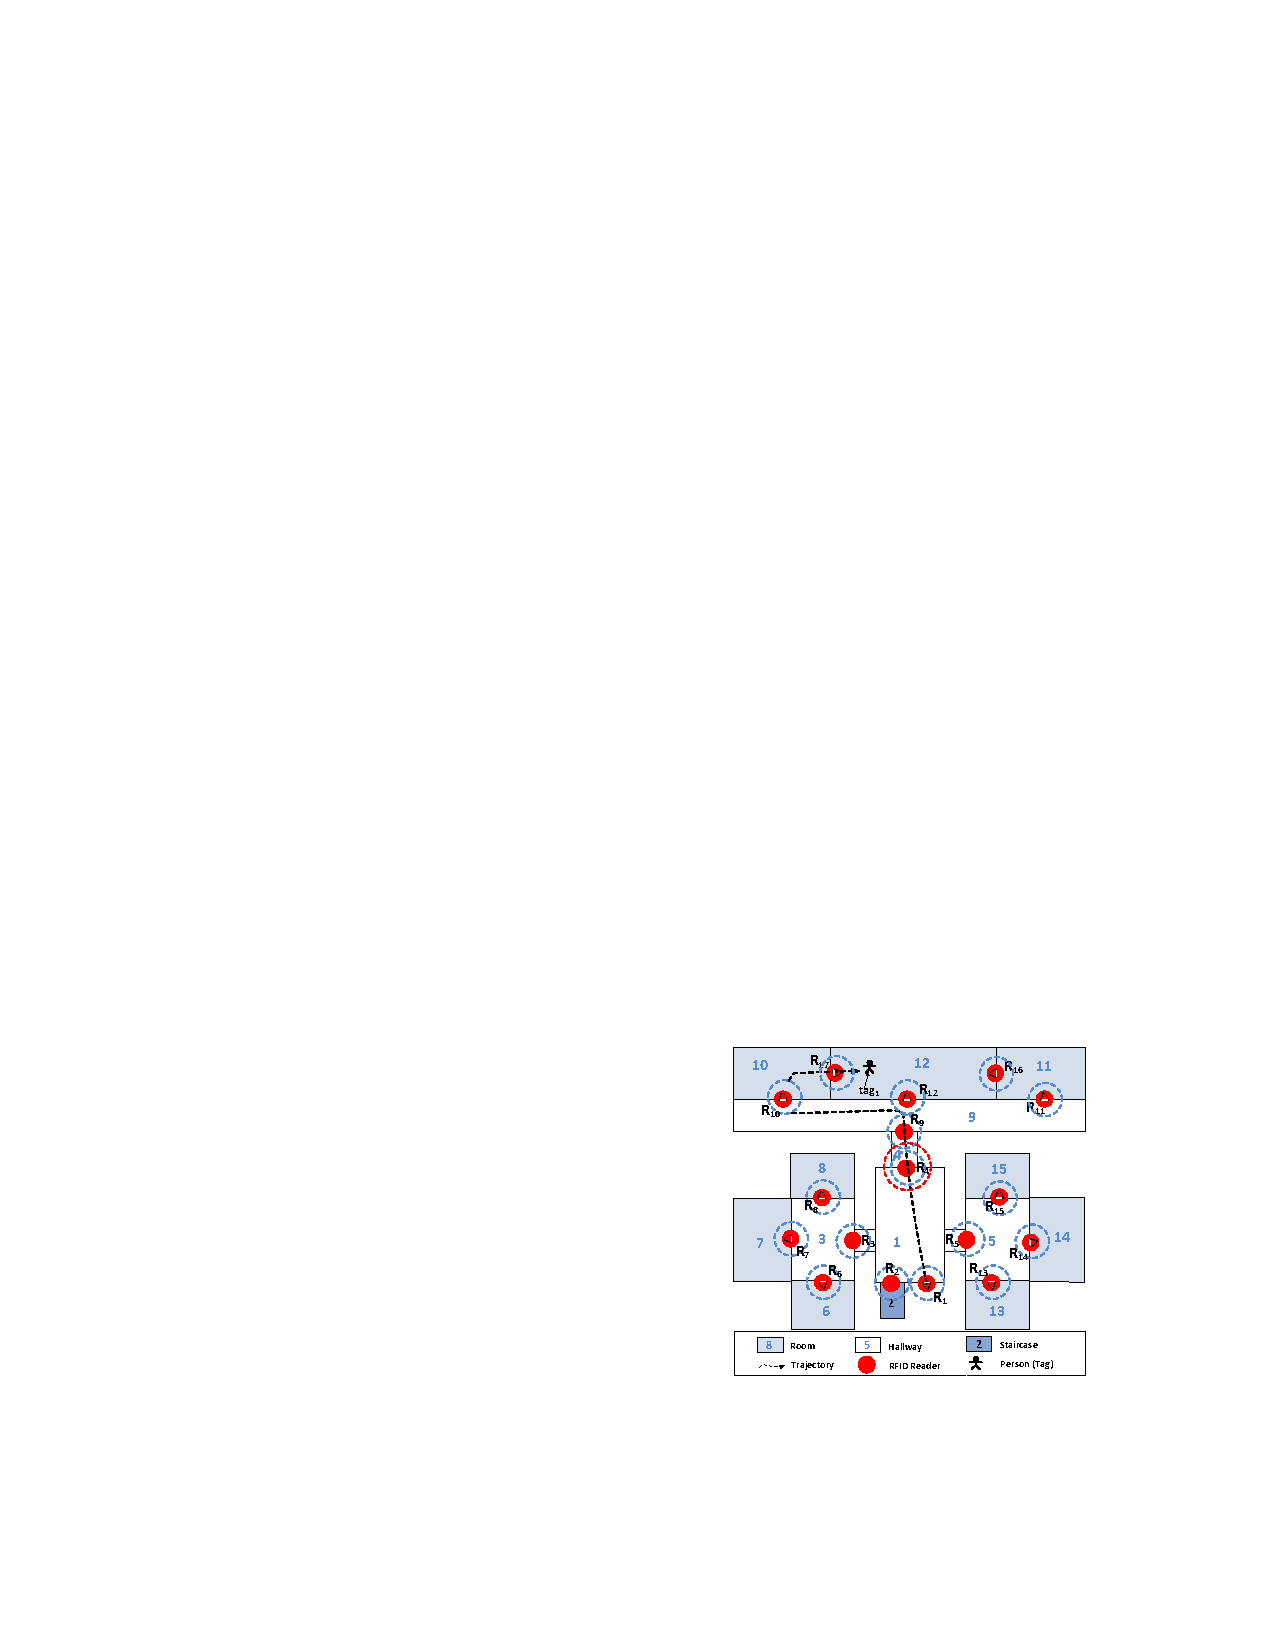
\includegraphics[width=\columnwidth]{figures/3-5/3-5-1.pdf}
  \end{figure}
  \ssize{\textit{an object with tag $tag_1$ moved into the building and was first detected by reader $R_1$ from time point $t_0$ to time point $t_3$, yielding four observations by reader $R_1$.}}

  \column{0.6\textwidth}
  \begin{figure}[tb]
    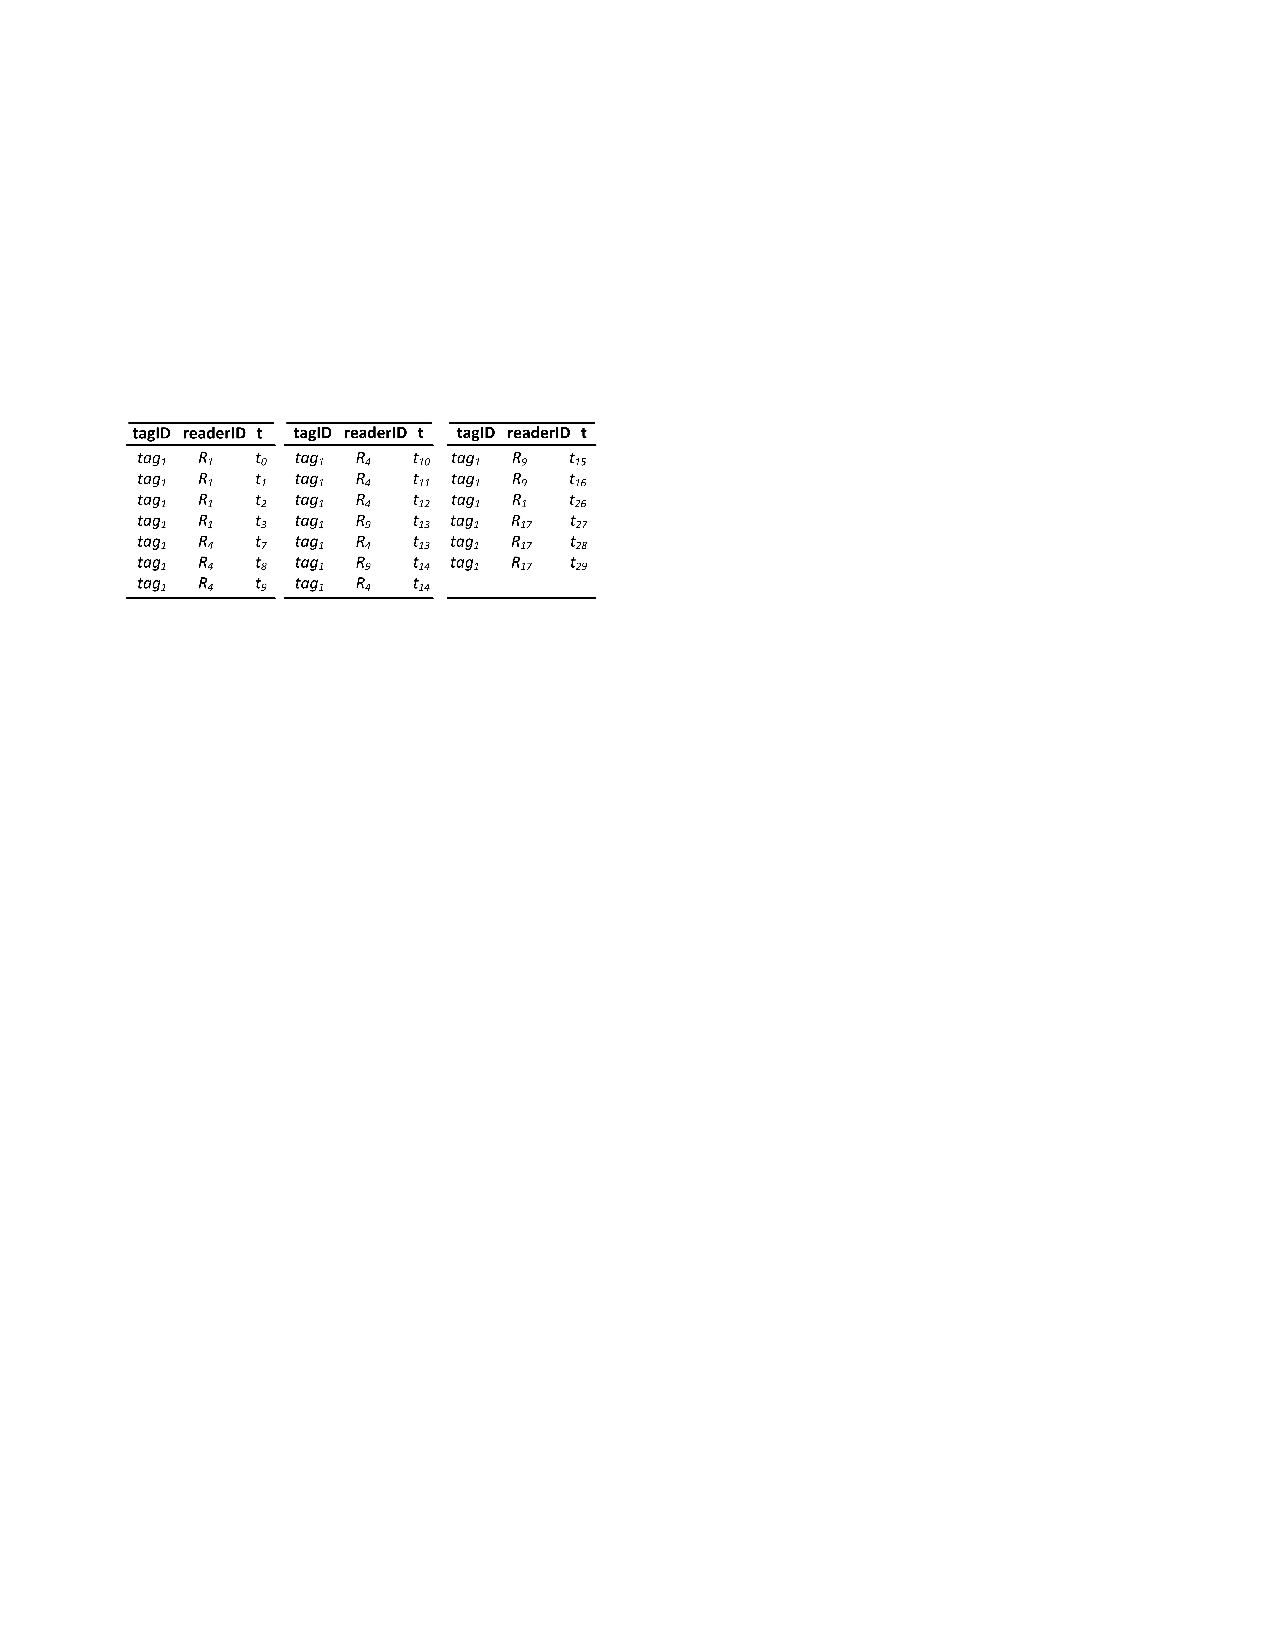
\includegraphics[width=\columnwidth]{figures/3-5/3-5-2.pdf}
  \end{figure}
  \ssize{
    1. at $t_{12}$ and $t_{13}$, $tag_1$ was detected by readers $R_4$ and $R_9$, it seems to be present in both locations, thus giving rise to a \emph{false positives}.\\~\\
    2. after $t_{16}$, $tag_1$ was detected by reader $R_{17}$ that kept detecting $tag_1$ until $t_{29}$. However $tag_1$ is not supposed to be detected by $R_{17}$ before it's detected by $R_{10}$. $tag_1$ passed through $R_{10}$ but failed to generate any information, giving rise to \emph{false negatives}.
  }

\end{columns}

\end{frame}

%------------------------------------------------

\begin{frame}
\frametitle{Motivation}

To support high-level RFID business logic processing, it is necessary to perform data cleansing to remove false negatives and false positives.\\~\\

Existing RFID data cleansing techniques require considerable specific prior knowledge for cleansing operations.

\begin{sitemize}
  \item to cleanse historical indoor RFID data, the graph model based cleansing approaches~\cite{baba2013spatiotemporal,baba2013graph,DBLP:conf/edbt/FazzingaFFP14} rely on graphs that capture the indoor topology, the deployment of readers, and multiple pertinet spatial-temporal properties.
  \item in the context of streaming RFID data, a probabilistic approach~\cite{tran2009probabilistic} demands to build four domain-specific probabilistic models before any data cleansing.
  \item also streaming RFID data, ~\cite{nie2009probabilistic} assumes that locations of neighboring objects are correlated to each other, lifting such assumptions and needs only minimal prior knowledge about indoor settings.
\end{sitemize}

\end{frame}

%------------------------------------------------

\begin{frame}
\frametitle{Preliminaries}

\ssize{\conceptbf{Hidden Markov Models} (HMMs) models two connected (discrete time) stochastic processes: an un-observed state transition process, and an observation process consisting of observable signals generated at each state. The underlying (hidden) state transition process is assumed to be Markovian and stationary.}

\begin{definition}[Hidden Markov Models]
  \ssize{
  An HMM is a tuple $\lambda = (\mathcal{S}, \mathcal{O}, A, B, \pi)$.
  \begin{enumerate}
    \item $\mathcal{S} = \{ s_1, ..., s_N \}$ is a set of (hidden) states.
    \item $\mathcal{O} = \{ 0_1, ..., o_K \}$ is a set of possible observations.
    \item $A$ is an $N \times N$ transition probability matrix:$A = (a_{ij})_{i,j=1,...,N}$, where $a_{ij}$ represents the transition probability form hidden state $s_i$ to hidden $s_j$.
    \item $B$ is an $N \times K$ observation probability matrix: $B = (b_{ih})_{i=1,...,N;h=1,...K}$, where $b_{ih}$ is the probability of ovserving $o_h$ when the hidden process is in state $s_i$.
    \item $\pi$ is a $N$-dimensional initial state probability vector: $\pi = (\pi_i)_{i=1,...,N}$, where $\pi_i$ is the probability that the hidden state process starts in state $s_i$.
  \end{enumerate}
  }
\end{definition}

\end{frame}

%------------------------------------------------

\begin{frame}
\frametitle{Preliminaries}

An HMM defines a discrete time stochastic process over the combined state and observation space $\mathcal{S} \times \mathcal{O}$. \\~\\

The state of the process at time $t$ is described by \emph{random variables} $S^{(t)}$ with values in $\mathcal{S}$, and $\mathcal{O}^{(t)}$ is defined by

\pause
\begin{equation}
  P(S^{(0)} = s_i) = \pi_i
\end{equation}

\pause
\begin{equation}
  P(S^{(t+1)} = s_j | S^{(t)} = s_i) = a_{ij}
\end{equation}

\pause
\begin{equation}
  P(o^{(t)} = o_h | S^{(t)} = s_i) = b_{ih}
\end{equation}

\end{frame}

%------------------------------------------------

\begin{frame}
\frametitle{Preliminaries}

For modeling processes where at each point in time observations of multiple variables are made, the basic HMM model have been generalized to \conceptbf{Multi-variate Hidden Markov Models}(MH-MMs).~\cite{kirshner2005modeling}.\\~\\

The simple observation space $\mathcal{O}$ is replaced by a multivariate observation space $\mathcal{O}_1 \times \hdots \times \mathcal{O}_M$, and at each time $t$ one observes variables $O^{(t)}_1,...,O^{(t)}_M$.\\~\\

One can furthermore introduce the assumption that the different observations are \emph{independent} given the hidden state, i.e.,

\pause

\begin{equation}
  P(O^{(t)}_1,...,O^{(t)}_M | S^{(t)}) = \prod_{i=1}^M P(O^{(t)}_i | S^{(t)})
\end{equation}

\end{frame}
